\documentclass[11pt]{article}
\usepackage{appendix}
\usepackage{graphicx} 
\usepackage{setspace}
\usepackage{amsmath,float,verbatim,multicol}
\usepackage{array}
\usepackage{lscape}
\usepackage{hyperref}

\usepackage{amssymb}
\bibliographystyle{plainnat}
\usepackage[round]{natbib}
\usepackage{multirow}

\setlength{\textheight}{8.8in} \setlength{\textwidth}{6.3in}
\setlength{\oddsidemargin}{0.2in} \setlength{\topmargin}{-0.30in}
\setlength{\footnotesep}{10.0pt}

\newcommand{\ol}{\overline}



\renewcommand{\baselinestretch}{1.25}
\title{Solving a Lifecycle Model}
\author{ Trevor Gallen \\ Econ 64200 }
\date{Fall 2022}

\begin{document}
\bibliographystyle{myplainnat}
%\bibpunct{(}{)}{;}{a}{}{,}6868

\maketitle

This homework is the first part of a multi-part homework.  This homework starts us with a relatively simple deterministic lifecycle model and asks you to solve it in Matlab.\\

\textbf{Deliverables}
\begin{itemize}
\item You should have a word/\LaTeX document that has three sections: 
\begin{enumerate}
\item Discusses the model and answers the questions I pose throughout.
\item Contains the tables and figures you will produce.
\item Contains a discussion of your programming choices if you had to make any.
\end{enumerate}
\item You should have a Matlab file or set of files (zipped) that contain \textbf{all} your programs and raw data.  There should be a file called ``Main.M" that produces everything I need in one click.
\end{itemize}


\section{Model}
Households have period utility over consumption $c_t$ and labor $L_t$ at time $t$: $u(c_t,L_t)$, which takes the form of balanced growth preferences with constant Frisch elasticity of labor supply:
$$u(c_t,L_t)=log(c_t)-\psi \frac{\epsilon}{1+\epsilon}L_t^{1+\epsilon}{\epsilon}$$
Letting $s$ denote savings, $w$ denote wages, $r$ denote interest rates, households have period budget constraint:
$$c_t+s_t=w_tL_t+(1+r_t)s_{t-1}$$
Households maximize the net present value of utility, discounted at a rate $0<\beta<1$. Assume that households live until period $T$.\\
\ \\
\textbf{Question 1a:} Write out the household's net present value budget constraint.\\
\ \\
\textbf{Suggested Sol}: Should look something like:
$$\sum_{t=1}^T\frac{c_t}{\prod_{\tau=1}^t(1+r_\tau)}-\sum_{t=1}^T\frac{w_tL_t}{\prod_{\tau=1}^t(1+r_\tau)}$$
Defining $r_1=0$.  Could also play with indicies.
\ \\
\textbf{Question 1b:} Write out the household's sequence problem.\\
 \ \\
\textbf{Suggested Sol}: Should look something like:
$$\underset{\{s_{t+1},c_t,L_t\}_{t=0}^\infty}{\max}\sum_{t=1}^T\beta^tu(c_t,L_t)$$
subject to:
$$c_t+s_t=w_tL_t+(1+r_t)s_{t-1}$$
With $s_{0}$ given.\ \\



\textbf{Question 1c:} Write out the household's value function problem.\\
 \ \\
\textbf{Suggested Sol}: Should look something like:
$$V_{t}(s_t,w_t,r_t)=\underset{\{s_{t+1},c_t,L_t\}}{\max}\left\{u(c_t,L_t)+\beta V_{t+1}(s_{t+1},w_{t+1},r_{t+1})\right\}$$
Note that because this is a lifecycle model, $t$ is also a state variable, with subscript.

\clearpage
\section{Basic Matlab}
Now, let the following numerical assumptions hold:
\begin{table}[ht!]
\centering
\begin{tabular}{lcc}
\hline
\hline
\multicolumn{3}{c}{Table 1: Calibration}\\
\hline
Concept & Parameter & Value \\ 
Lifespan & T & 45 \\
Disutility of labor & $\psi$ & 10\\
Frisch elasticity of labor supply & $\epsilon$ & 0.75\\
Discount factor & $\beta$ & 0.96\\
Wages: $w_t$, $t\neq 30$ & $w_{t\neq30}$ & 1\\
Wages: $w_30$ & $w_{t\neq30}$ & 1.05\\
Interest rates: $r_t$, $t\neq 20$ & $r_{t\neq30}$ & 0.05\\
Interest rates $r_20$ & $w_{t\neq20}$ & 1.1\\
\hline
\hline
\end{tabular}
\end{table}

\textbf{Question 2:} Write a Matlab program that does the following.
\begin{itemize}
\item Section 1a:  Defines all exogenous parameters in Table 1, including making $w_t$ and $r_t$ 45-entry column vectors. (It is important to be consistent in terms of column vs. row).
\item Section 1b:  Defines a NPV discount rate for all 45 periods (e.g. contains $[1;1/(1+r_1) ;1/((1+r_1)*(1+r_2))] $and so on.  You may find Matlab's cumulative product function ``cumprod" useful.
\item Section 2a:  Define the utility function, which takes in $c$ and $L$ (as inputs) and spits out utility (given $\psi$ and $\epsilon$, which are set by Table 1.  Write it so you can give the function a vector of $c$ and $L$ and it will spit out a vector of utilities.
$$ut(c,L)=log(c_t)-\psi \frac{\epsilon}{1+\epsilon}L_t^{1+\epsilon}{\epsilon}$$
\item Section 2b:  A function of the lifetime excess savings, which takes in a vector of $c_t$'s and a vector of $w_t$'s and $L_t$'s, and spits out excess savings
$$bc\_lifetime(c,L)=\sum_{t=1}^T\frac{c_t}{\prod_{\tau=1}^t(1+r_\tau)}-\sum_{t=1}^T\frac{w_tL_t}{\prod_{\tau=1}^t(1+r_\tau)}$$
\item Section 2c:  A lifetime utility function which penalizes debt (a simple way of making constrained optimization unconstrained), e.g.:
$$ut\_lifetime(c,L) = sum(beta.^[0:T-1]ut(c,L))-10*(bc\_lifetime(c,L)>0)*bc\_lifetime(c,L)$$
\item Section 3:  Create an initial guess, and pass the negative of the life to a \emph{minimizer}, such as fminunc.  You may have to think about how to pass the anonymous arguments.
\item Section 4:  Graph out $c_t$ and $L_t$.  Clearly label your graphs.
\item Section 5:  Answer the following questions:
\begin{itemize}
\item What is the intertemporal elasticity of substitution suggested by consumption's response in period 20?  
\item What is the Frisch elasticity of labor supply suggested by labor's response in period 30?
\item Why is consumption rising over time?  
\item What, in the calibration and functional form choice drove the numerical answers to the previous three questions?  What parameterization of $\beta$ would make $c_{t+1}/c_t$ flat?
\end{itemize}
\end{itemize}

\textbf{Suggested Sol}: See Hwk1Sol.m
Below, I plot the results:
\begin{figure}[ht!]
\centering
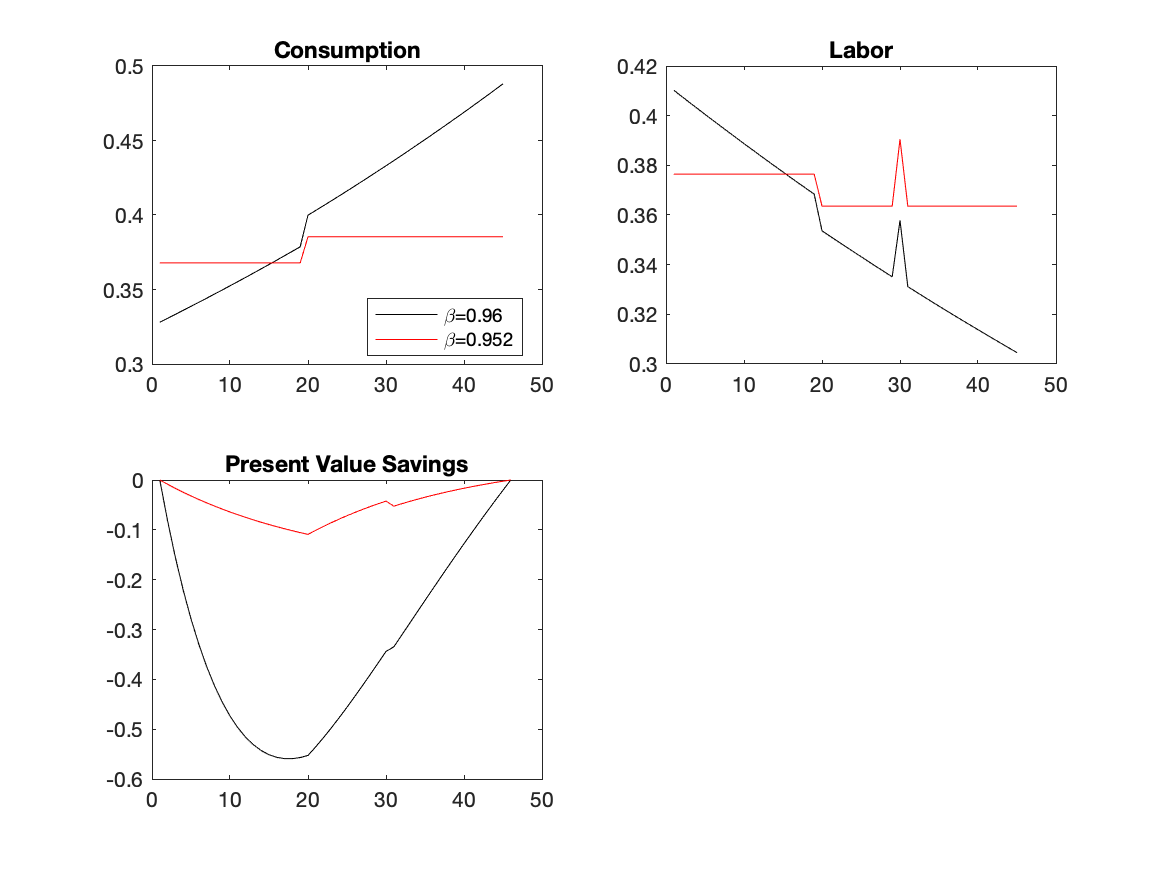
\includegraphics[scale=0.5]{Figure1.png}
\caption{Consumption, labor, and savings for $\beta=0.96$ and $\beta=0.952$}
\end{figure}
Some interesting takeaways:
\begin{itemize}
\item The intertemporal elasticity of substitution can be calculated by knowing one convenient definition:
$$\sigma=-\frac{d \log\left(\frac{c_{t+1}}{c_t}\right)}{dr}$$
Put simply, the percentage change in consumption growth due to a percentage point change in interest rates.  When there is no trend ($\beta=0.952$) then we can just calculate the percent change: 0.385/0.368-1=0.046, divided by the interest rate change of 0.05 is 0.92, close to the one that log preferences would predict.  If there is a trend, then we have to difference it out:  (0.40/0.379)-(0.379/0.376)=0.047, or $\sigma=0.94$.  
\item The Frisch elasticity of substitution is also quite close to the calibrated value.  For no trend, wages went up by 10\%, while labor went up by (0.358/0.335)=0.074, for a Frisch elasticity of 0.74, close to the 0.75 the preferences would predict (in a perfect experiment).  When $\beta=0.96$, we take out the labor trend (-0.6\% decline), so that the 6.8\% increase is really a 0.074\% increase, giving again a Frisch elasticity of 0.75.
\item Consumption goes up because the Euler equation is:
$$\frac{c_{t+1}}{c_{t}}=\beta(1+r_{t+1})$$
If your indexing was different so that consumption in the first period was discounted by interest rates but utility wasn't multiplied by $\beta$, you might have had a different trend.
\end{itemize}


\begin{table}[ht!]
\centering
\begin{tabular}{lcclllcc}
\multicolumn{8}{c}{Table 2: Consumption  and Labor}\\
\hline\hline
\multicolumn{3}{c}{Consumption  } & & &  \multicolumn{3}{c}{Labor}\\
Time & $\beta=0.96$ & $\beta=0.952$ & \ \  & \ \ & Time & $\beta=0.96$ & $\beta=0.952$\\
\cline{1-3}  \cline{6-8}
 $c_{18}$ & 0.376 & 0.368  & & &  $L_{28}$ & 0.337  & 0.364\\
$c_{19}$ & 0.379& 0.368  & & & $L_{29}$ & 0.335 & 0.364\\
$c_{20}$ & 0.400 & 0.385  & & &  $L_{30}$ & 0.358 & 0.391\\
\hline\hline
\end{tabular}
\end{table}



\clearpage
\section{Research}
You now have a very simple deterministic numerical model of people's labor over the lifecycle.  However, the model is too simple to be particularly interesting.  Change the model in an interesting way, and report your results.  This is your opportunity to actually think, so please take time with this:  how can you adjust the model, parameterization, etc. to make this model (a) more interesting and (b) more realistic?\\
\ \\
\textbf{Suggested Sol}: Many possibilities!  One is to include ``learning by doing."  I did so in a primitive way by making the change in wage equal to the cumulative hours spent working divided by 10, minus a quadratic trend denoting declining labor productivity at older ages.  When I do so (with $\beta=0.952$) I get flat consumption, a u-shaped labor supply (at first age-related depreciation is small, so learning by doing dominates, then it rises).  I then get a u-shaped lifetime labor curve.

\begin{figure}[ht!]
\centering
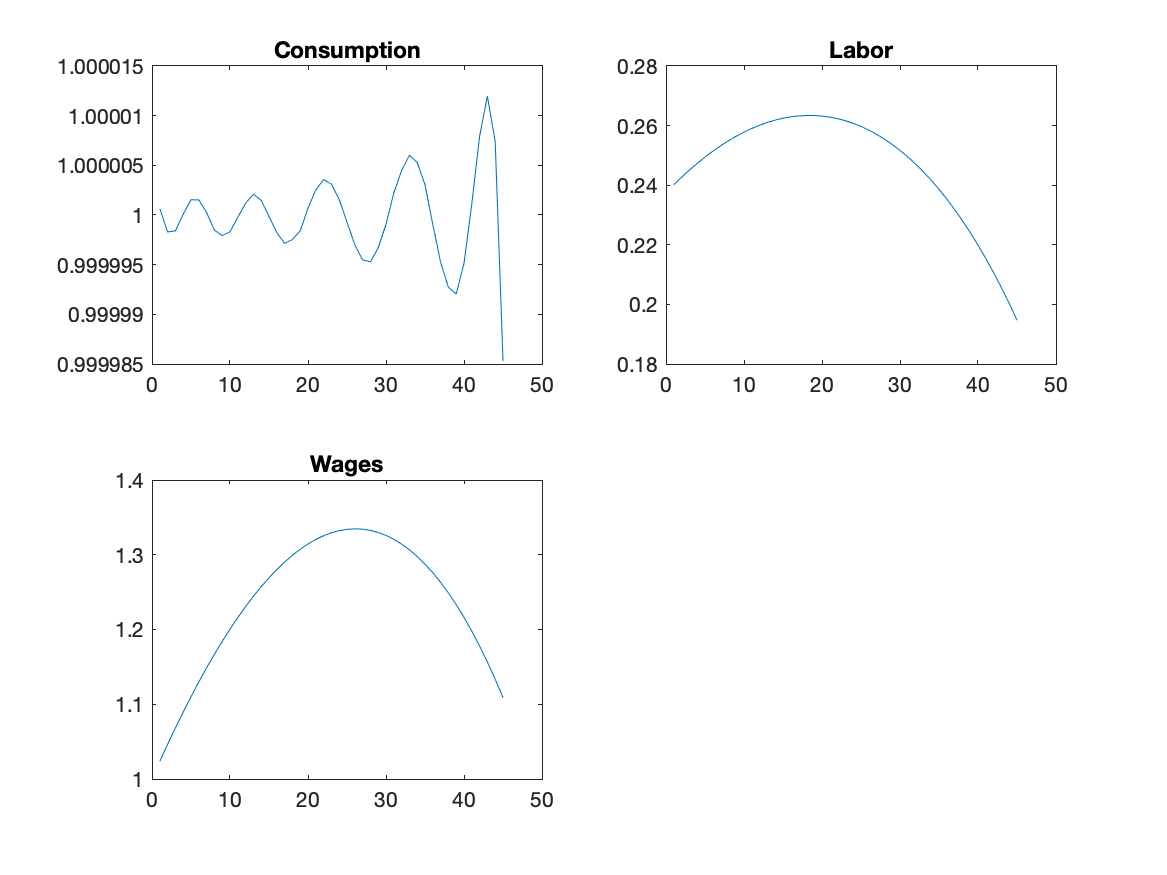
\includegraphics[scale=0.5]{Figure2.png}
\caption{Consumption, labor, and wages in a learning-by-doing model}
\end{figure}


\end{document}





